\documentclass[twocolumn,11pt,a4paper]{article}

% ======================================================================
%  A COORDINATE THEORY OF ADVERTISING
%  Bounded Receivers, Action-Cells, and the Calculus of Decoder-Shifts
%
%  Self-contained. No reliance on unpublished work; all citations are to
%  standard, externally published literature.
% ======================================================================

\usepackage[utf8]{inputenc}
\usepackage[T1]{fontenc}
\usepackage{lmodern}
\usepackage[a4paper,margin=2cm]{geometry}
\usepackage{amsmath,amssymb,amsthm,mathtools}
\usepackage{bm}
\usepackage{graphicx}
\usepackage{enumitem}
\usepackage{booktabs}
\usepackage{array}
\usepackage{microtype}
\usepackage{xcolor}
\usepackage[colorlinks=true,linkcolor=blue!45!black,citecolor=blue!45!black,
            urlcolor=blue!45!black]{hyperref}
\usepackage[round]{natbib}

% ---- theorem environments ----
\newtheoremstyle{adv}{6pt}{6pt}{\itshape}{}{\bfseries}{.}{.5em}{}
\theoremstyle{adv}
\newtheorem{theorem}{Theorem}[section]
\newtheorem{lemma}[theorem]{Lemma}
\newtheorem{proposition}[theorem]{Proposition}
\newtheorem{corollary}[theorem]{Corollary}

\theoremstyle{definition}
\newtheorem{definition}[theorem]{Definition}
\newtheorem{axiom}{Axiom}
\newtheorem{principle}[theorem]{Principle}
\newtheorem{example}[theorem]{Example}

\theoremstyle{remark}
\newtheorem{remark}[theorem]{Remark}

% ---- macros ----
\newcommand{\Real}{\mathbb{R}}
\newcommand{\Nat}{\mathbb{N}}
\newcommand{\Out}{\mathcal{X}}         % outcome / percept space
\newcommand{\Know}{\mathcal{K}}        % knowledge framework
\newcommand{\Acts}{\mathcal{Y}}        % action space
\newcommand{\Cell}{\mathcal{C}}        % action-cell
\newcommand{\Dec}{D}                   % decoder
\newcommand{\Proj}{\Pi}                % candidate projection
\newcommand{\Recv}{R}                  % receiver
\newcommand{\Sval}{S}                  % S-functional
\newcommand{\floor}{\beta}            % receiver floor
\newcommand{\tol}{\tau}               % cell tolerance
\newcommand{\Eff}{\varepsilon}        % an effect
\newcommand{\Carrier}{\kappa}         % carrier (overloaded? use \mathsf)
\renewcommand{\Carrier}{\mathsf{c}}
\newcommand{\Mean}{\mathcal{M}}        % meaning space
\newcommand{\shift}{\Delta}            % decoder-shift
\newcommand{\pot}{\kappa}             % catalytic power
\newcommand{\Adv}{\mathcal{A}}        % advert
\newcommand{\dist}{d}
\newcommand{\Sig}{\Sigma}
\newcommand{\target}{x^{\dagger}}     % target percept (in cell)
\newcommand{\half}{\tfrac{1}{2}}

\title{\bfseries A Coordinate Theory of Advertising:\\
Bounded Receivers, Action-Cells, and the\\
Calculus of Decoder-Shifts}

\author{%
  \normalsize Pugachev Cobra Project --- Working Paper\\
  \small \texttt{advertising-coordinate-receivers}
}
\date{\today}

\begin{document}
\maketitle

\begin{abstract}
\noindent
We develop a mathematical theory of advertising from a single primitive:
the \emph{bounded receiver}, a finite cognitive system that decodes
percepts into an internal representation and projects that representation
back onto a space of practical actions. We prove, as theorems rather than
assumptions, that (i) a bounded receiver cannot resolve outcomes to
arbitrary precision---there is a strictly positive \emph{floor} on
residual semantic distance; (ii) the operational unit of value is
therefore not a point but an \emph{action-cell}, a positive-tolerance
region of percept space whose members are behaviourally
indistinguishable; and (iii) consequently the object an advertisement
acts upon is not the product nor the percept but the receiver's
\emph{decoder}---the map from percept to meaning. We formalise an advert
as a finite composition of \emph{effects}, each a pair $(\Carrier,\shift)$
of a physical carrier and a \emph{decoder-shift}: a movement the carrier
induces in meaning-space, expressed relative to action-cells. We prove a
\emph{Decoupling Theorem} separating an effect's carrier (its pixels and
sound) from its semantic action (the cell it moves the receiver toward),
showing the two are distinct representations of one object rather than
cause and annotation. We derive a \emph{multiplicative law of persuasive
power} under which the power of a stack of effects composes as
$1-\prod_i(1-\pot_i)$, yielding closed-form predictions for diminishing
returns, frequency saturation, and the impossibility of total persuasion.
We prove that an advert's elements must form a \emph{coherent support
structure} (a strongly connected agreement graph of at least three
elements) and that incoherence is detectable from ordinal data alone. We
recover, as corollaries, the informational and persuasive views of
advertising, the central/peripheral route distinction, framing effects,
mere-exposure saturation, and the structural limit on signalling. The
theory is \emph{ordinal}: it asserts cell-membership and comparisons
between effects, never absolute magnitudes, in accordance with the floor
theorem which forbids point-valued meaning. We close by stating the
theory as a compilation target: an advert is a typed program whose
semantics is a decoder-shift toward a target action-cell, and whose
correctness is the coherence of that shift.
\end{abstract}

% ======================================================================
\section{Introduction}
\label{sec:intro}
% ======================================================================

\subsection{The question}

What is an advertisement? The question is older than its discipline, and
the answers cleave into two traditions. The \emph{informational} view
holds that advertising transmits facts---price, availability, quality---
that rational consumers incorporate into their decisions
\citep{stigler1961,nelson1974,milgrom1986}. The \emph{persuasive} view
holds that advertising alters preferences directly, manufacturing wants
that did not previously exist \citep{dixit1978,bagwell2007}. A third,
\emph{complementary}, view treats the advertisement as a good that enters
utility alongside the product \citep{becker1993}.\footnote{We discuss the
relation to these traditions throughout; our aim is not to adjudicate
between them but to exhibit a single structure of which each is a
projection.} Each tradition has empirical support and each has anomalies
it cannot absorb. The informational view cannot explain why a wordless
image of a sun-drenched landscape sells liquor; no fact is transmitted.
The persuasive view cannot say what, precisely, is altered, nor why the
same advertisement moves one viewer and leaves another unmoved.

We propose that both traditions describe projections of a single object,
and that the object becomes visible only when one begins not from the
product, nor from the message, but from the \emph{receiver}: the bounded,
finite cognitive system that must decode whatever arrives and act on it.

\subsection{The thesis in one paragraph}

A receiver is finite. It cannot represent every distinguishable state of
the world; it has a fixed, bounded internal vocabulary. From finiteness
alone we will prove that the receiver can never align perfectly with any
target---there is an irreducible floor on how precisely it can resolve a
percept. The immediate consequence is that practical meaning is granular:
what a receiver \emph{does} partitions the world into cells of
behaviourally equivalent percepts, and the unit of value is the cell, not
the point. An advertisement, then, cannot transmit a point (no bounded
receiver could receive it) and cannot install a preference (preferences
are themselves cell-structured). What it can do, and the only thing it can
do, is shift the receiver's \emph{decoder}: the map that assigns each
percept to a cell. ``Make the bottle read as authentic'' is a decoder-
shift; ``feels shot in Mexico'' names a region of meaning-space toward
which an effect moves the decoder; ``best for liquor'' asserts that this
region has high affinity with the purchase-cell for liquor. We will make
each of these statements precise, prove the laws they obey, and show that
the resulting calculus is ordinal---it speaks of cells and comparisons,
never of magnitudes the floor theorem forbids.

\subsection{Contributions}

\begin{enumerate}[leftmargin=1.4em,itemsep=2pt]
\item \textbf{The receiver primitive and the Floor Theorem}
  (\S\ref{sec:receiver}). We define the bounded receiver and prove it has
  a strictly positive resolution floor $\floor>0$; perfect alignment is
  impossible for any finite agent.
\item \textbf{Cell-truth} (\S\ref{sec:cells}). We prove that practical
  meaning is a positive-tolerance cell and that all percepts within a cell
  are receiver-indistinguishable. Value is cell-valued.
\item \textbf{The decoder as the locus of advertising}
  (\S\ref{sec:decoder}). We prove that, holding the product fixed, the
  only quantity an advertisement can change is the decoder, and we
  characterise the three exhaustive mechanisms by which it can do so.
\item \textbf{Effects as carrier--shift pairs and the Decoupling Theorem}
  (\S\ref{sec:effects}). We define an effect, prove that its carrier and
  its semantic shift are independent up to a representation equivalence,
  and formalise the ``advert unit.''
\item \textbf{The multiplicative law of persuasive power}
  (\S\ref{sec:power}). We derive the composition law for stacks of
  effects, with corollaries on diminishing returns, frequency saturation,
  and the impossibility of total persuasion.
\item \textbf{Coherence} (\S\ref{sec:coherence}). We prove that effective
  adverts require a coherent support structure of size $\ge 3$ and that
  incoherence is ordinally detectable---the basis of an automated critic.
\item \textbf{Recovery of the classical views} (\S\ref{sec:recovery}).
  We recover the informational, persuasive, dual-route, framing,
  mere-exposure, and signalling accounts as corollaries or limiting cases.
\end{enumerate}

The theory is deliberately substrate-neutral and ordinal. It does not
predict that any particular advertisement will perform better; it
specifies what an advertisement \emph{is}, what it can and cannot do, and
which of its internal structures are necessary for it to do anything at
all.

% ======================================================================
\section{The Bounded Receiver}
\label{sec:receiver}
% ======================================================================

\begin{figure*}[t]
\centering
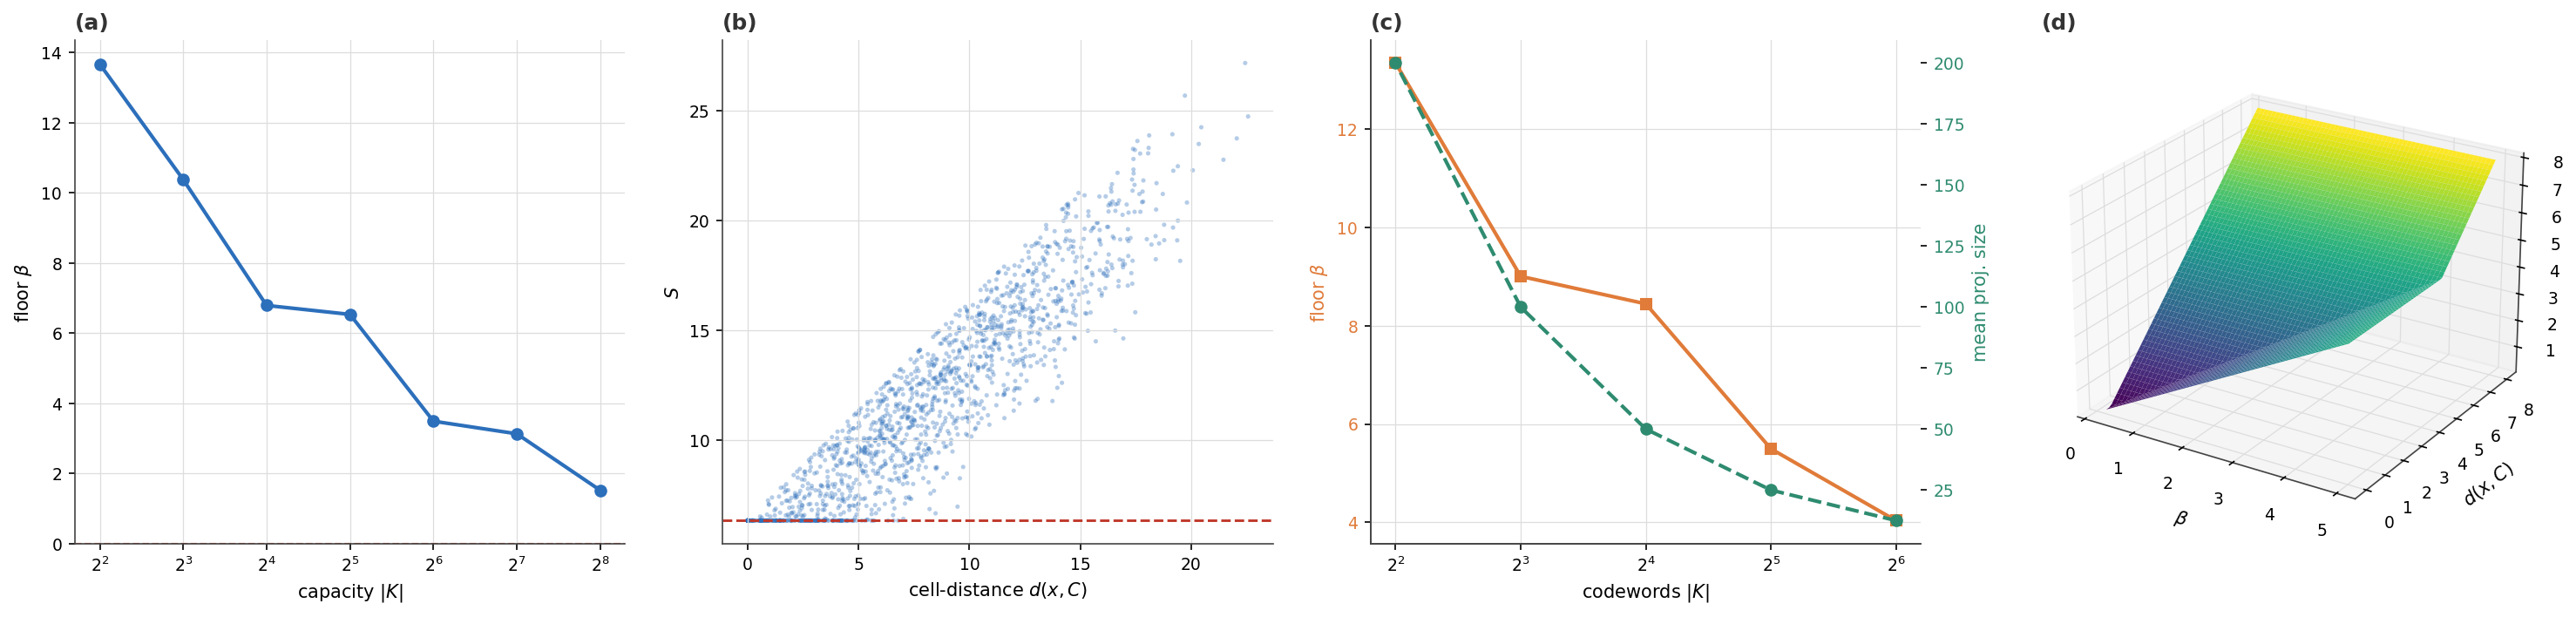
\includegraphics[width=\textwidth]{panels/panel_1.png}
\caption{\textbf{The Floor.} Bounded receivers cannot resolve a percept to a
point. (a)~The floor $\floor$ falls as codebook capacity $|\Know|$ grows but
stays strictly positive. (b)~Semantic distance $\Sval$ never drops below
$\floor$ across thousands of evaluations. (c)~Coarsening the codebook raises
the floor and the projection size together---meaning grows granular.
(d)~The $S$-surface $\Sval(\floor,\dist)=\max(\floor,\dist)+\!$floor offset:
a floor-plateau over a distance-cone.}
\label{fig:panel1}
\end{figure*}

\subsection{Percepts, knowledge, and action}

We begin with three spaces and three axioms. The axioms are not
idealisations to be relaxed later; they are the minimal conditions under
which a cognitive system is finite and embodied, and every subsequent
theorem is a consequence of them.

\begin{definition}[Percept space]
\label{def:percept}
A \emph{percept space} is a triple $(\Out,\dist,\Sig)$ where $\Out$ is a
non-empty set of percepts (the totality of audiovisual configurations a
viewer might be presented with), $\dist:\Out\times\Out\to[0,\Sig]$ is a
bounded pseudometric (a notion of perceptual dissimilarity satisfying
$\dist(x,x)=0$, symmetry, and the triangle inequality), and
$\Sig\in(0,\infty)$ is the maximal semantic distance. The canonical
normalisation is $\Sig=100$; no result depends on the value.
\end{definition}

\begin{definition}[Action space and action map]
\label{def:action}
An \emph{action space} $(\Acts,\dist_\Acts)$ is a metric space of
practical responses (buy, ignore, share, distrust, $\dots$). An
\emph{action map} is a measurable surjection
$\Act:\Out\to\Acts$ assigning to each percept the practical response it
elicits.
\end{definition}

\begin{axiom}[Bounded representation]
\label{ax:bounded}
A receiver's internal vocabulary is a set $\Know$ of finite cardinality
(or, in the infinite idealisation, of cardinality strictly less than
$|\Out|$). The receiver cannot hold a distinct internal token for every
distinguishable percept.
\end{axiom}

\begin{axiom}[No null state]
\label{ax:null}
At every instant the receiver occupies exactly one internal state; there
is no ``blank'' or ``undefined'' percept. Decoding is total.
\end{axiom}

\begin{axiom}[Finite resolution]
\label{ax:resolution}
Every act of perception has finite resolution $\delta>0$: percepts closer
than $\delta$ in $\dist$ are not distinguished.
\end{axiom}

Axiom~\ref{ax:bounded} is finiteness of memory; Axiom~\ref{ax:null} is the
embodied fact that a living perceiver is always in \emph{some} state;
Axiom~\ref{ax:resolution} is the finite acuity of any sense organ or
measuring instrument. They are satisfied by human viewers, by animals, and
by any physical machine.

\begin{definition}[Receiver]
\label{def:receiver}
A \emph{receiver} over $(\Out,\dist,\Sig)$ is a quadruple
$\Recv=(\Know,\Dec,\Proj,\floor)$ where
\begin{enumerate}[label=(\roman*),leftmargin=1.8em,itemsep=1pt]
\item $\Know$ is the \emph{knowledge framework} (Axiom~\ref{ax:bounded});
\item $\Dec:\Out\to\Know$ is the \emph{decoder}, a measurable map sending
  each percept to an internal representation (this is \emph{perception});
\item $\Proj:\Know\to 2^{\Out}\setminus\{\varnothing\}$ is the
  \emph{candidate projection}, sending each representation to the set of
  percepts compatible with it (this is \emph{inference}), and satisfying
  the consistency condition $\Dec(x)\in\Dec(\Proj(\Dec(x)))$ for all $x$;
\item $\floor\in(0,\Sig]$ is the \emph{noise floor},
  \[
    \floor \;=\; \sup_{x\in\Out}\;\inf_{x'\in\Proj(\Dec(x))}\dist(x,x'),
  \]
  the worst-case irreducible gap between a percept and the nearest percept
  the receiver can reconstruct from its representation of it.
\end{enumerate}
\end{definition}

The four components separate concerns usually conflated. $\Dec$ is what
the viewer sees \emph{as}; $\Proj$ is what they infer could be the case;
$\floor$ is the residue that survives both. We now show $\floor>0$ is
forced.

\subsection{The $S$-functional and the Floor Theorem}

\begin{definition}[$S$-functional]
\label{def:sfunctional}
For a receiver $\Recv$, a percept $x$, and a target region
$\Cell\subseteq\Out$, the \emph{semantic distance} of $x$ to $\Cell$ is
\[
  \Sval(\Recv,x;\Cell)\;=\;\inf_{x'\in\Proj(\Dec(x))}\dist(x',\Cell)\;+\;\floor,
\]
where $\dist(x',\Cell)=\inf_{c\in\Cell}\dist(x',c)$.
\end{definition}

$\Sval$ measures how far, after decoding and inference, the receiver
remains from registering $x$ as a member of $\Cell$. The additive $\floor$
encodes that even a perfectly placed percept is registered only up to the
receiver's irreducible noise.

\begin{theorem}[Floor Theorem]
\label{thm:floor}
For every bounded receiver $\Recv$, $\floor>0$, and for every percept $x$
and region $\Cell$,
\[
  \Sval(\Recv,x;\Cell)\;\ge\;\floor\;>\;0.
\]
No bounded receiver attains $\Sval=0$: perfect semantic alignment is
impossible.
\end{theorem}

\begin{proof}
Suppose $\floor=0$. Then for every $\eta>0$ and every $x$ there is
$x'\in\Proj(\Dec(x))$ with $\dist(x,x')<\eta$; taking $\eta\to0$ forces
$\Proj(\Dec(x))$ to determine $x$ uniquely up to $\dist$-distance $0$, i.e.
the composite $\Proj\circ\Dec$ is injective on $\dist$-classes. An
injection from $\Out$'s distinguishable classes into $\Know$ contradicts
Axiom~\ref{ax:bounded} ($|\Know|<|\Out|$) whenever $\Out$ has more
distinguishable classes than $\Know$ has tokens, which Axiom~\ref{ax:resolution}
guarantees is the generic case (the number of $\delta$-separated classes is
$|\Out|$-large). Hence $\floor>0$. The displayed bound is then immediate
from Definition~\ref{def:sfunctional}, since the infimum term is
non-negative.
\end{proof}

\begin{corollary}[No perfect persuasion]
\label{cor:noperfect}
There is no advertisement, however constructed, that drives a bounded
receiver's semantic distance to a target to zero. Residual distance at
least $\floor$ always remains. Persuasion is bounded below by the
receiver's own finiteness, not by any defect of the message.
\end{corollary}

\begin{remark}
Corollary~\ref{cor:noperfect} is not pessimism; it is the precise
statement of why a ``perfect ad'' is a category error, and why the
relevant objective is never alignment to a point but \emph{entry into a
cell}, defined next. It is the advertising form of bounded rationality
\citep{simon1955,simon1956,gigerenzer1996}: the limit is structural.
\end{remark}

% ======================================================================
\section{Cell-Truth: Value Is a Region}
\label{sec:cells}
% ======================================================================

\begin{figure*}[t]
\centering
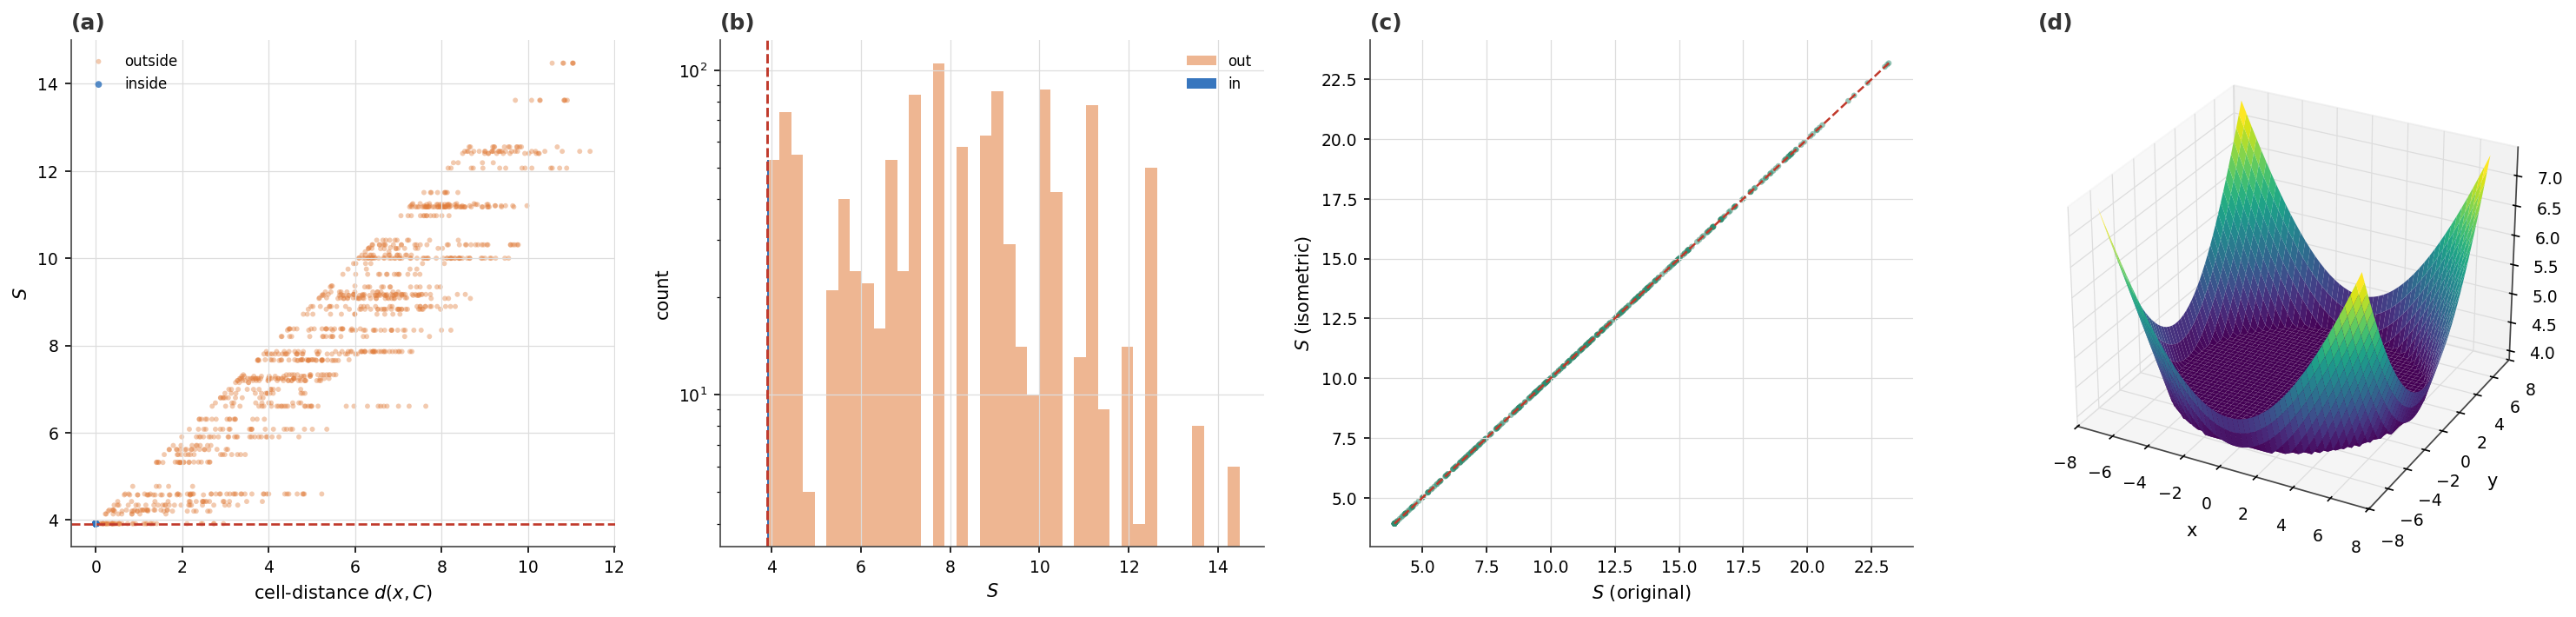
\includegraphics[width=\textwidth]{panels/panel_2.png}
\caption{\textbf{Cell-Truth and invariance.} (a)~$\Sval$ versus cell-distance:
flat at $\floor$ inside the cell, rising linearly outside---in-cell percepts
are indistinguishable. (b)~Histogram of in-cell $\Sval$ values: a spike
exactly at $\floor$ (zero spread), with out-of-cell values strictly above.
(c)~$\Sval$ under isometric re-encoding lands on the identity diagonal to
machine precision (invariance). (d)~The two-dimensional $\Sval$ field over
percept space: a flat-bottomed bowl whose base is the action-cell.}
\label{fig:panel2}
\end{figure*}

\subsection{Action-cells}

\begin{definition}[Action-cell]
\label{def:cell}
For $y\in\Acts$, the \emph{action-cell} of $y$ is the preimage
$\Cell_y=\Act^{-1}(\{y\})\subseteq\Out$. We equip it with
\begin{itemize}[leftmargin=1.4em,itemsep=1pt]
\item \emph{tolerance} $\tol(\Cell_y)=\sup_{x\in\Out}\inf_{c\in\Cell_y}\dist(x,c)>0$,
\item \emph{cell-distance} $\dist(x,\Cell_y)=\inf_{c\in\Cell_y}\dist(x,c)$.
\end{itemize}
A \emph{generic action-cell} is any nonempty $\Cell\subseteq\Out$ with
$\tol(\Cell)>0$ and finite diameter below $\Sig$.
\end{definition}

The cell $\Cell_{\text{buy-liquor}}$ is the set of all percepts that
trigger the purchase response for a liquor brand---every configuration of
imagery, sound, and framing that makes a viewer reach for the bottle. It
is a region, not a point, because many distinct percepts trigger the same
response.

\begin{theorem}[Cell-Truth]
\label{thm:celltruth}
Let $\Cell_y$ be an action-cell with $\tol(\Cell_y)>0$. For any receiver
$\Recv$ and any two percepts $x_1,x_2\in\Cell_y$,
\[
  \Sval(\Recv,x_1;\Cell_y)=\Sval(\Recv,x_2;\Cell_y)=\floor.
\]
All percepts within a cell are receiver-indistinguishable.
\end{theorem}

\begin{proof}
For $x_i\in\Cell_y$, $\dist(x_i,\Cell_y)=0$, so the infimum term in
Definition~\ref{def:sfunctional} is at most $0$, giving
$\Sval\le\floor$; the Floor Theorem gives $\Sval\ge\floor$. Hence equality.
\end{proof}

\begin{principle}[Operational meaning is granular]
\label{prin:granular}
For a bounded receiver, what an advertisement \emph{means} is the cell its
percept falls into, not the percept itself. Two adverts that place the
viewer in the same cell are operationally equivalent however different
they look; two that look identical but fall in different cells mean
different things.
\end{principle}

This is the formal content of the long-standing observation that what
matters in advertising is the response evoked, not the literal content
\citep{krugman1965,vakratsas1999}. It also dissolves the informational
view's puzzle: the sun-drenched landscape transmits no fact, yet places
the viewer in $\Cell_{\text{buy-liquor}}$, and by
Principle~\ref{prin:granular} that placement \emph{is} its meaning.

\subsection{Value is cell-valued; point-value is forbidden}

\begin{definition}[Point-value and cell-value]
\label{def:pointvalue}
A receiver \emph{carries point-value} if for every $x$, $\Proj(\Dec(x))$
is a singleton (the receiver resolves percepts to points). The
\emph{cell-value} of $x$ is the action-cell $\Cell_{\Act(x)}$ containing
it.
\end{definition}

\begin{theorem}[Point-value is forbidden]
\label{thm:nopoint}
No bounded receiver carries point-value. Consequently, no theory of
advertising effect can rest on a point-valued utility or quality scale;
all value is cell-value.
\end{theorem}

\begin{proof}
If $\Proj(\Dec(x))=\{x\}$ for all $x$, then
$\inf_{x'\in\Proj(\Dec(x))}\dist(x,x')=0$ for all $x$, forcing $\floor=0$
and contradicting the Floor Theorem. Hence $\Proj(\Dec(x))$ is non-
singleton for some $x$; value resolves only to cells.
\end{proof}

\begin{remark}[The granularity of price]
\label{rem:price}
The same argument applied to a price percept makes a ``price'' a band, not
a number: a viewer registers ``about twenty dollars,'' a cell of tolerance
$\floor$, not the point $\$19.99$. The cent-precise sticker is a carrier
whose decoded value is a cell. Willingness-to-pay is then the slack
$\tol(\Cell)-\floor$ between the width of the price-cell and the floor:
positive exactly when the viewer can be brought inside the cell. We use
this in \S\ref{sec:recovery}.
\end{remark}

\subsection{Representational invariance}

\begin{theorem}[Representational invariance]
\label{thm:repinv}
Let $\varphi:\Out\to\Out'$ be an isometric bijection between percept
spaces, and let $\Recv'$ be the receiver transported along $\varphi$. Then
for all $x$ and $\Cell$,
$\Sval(\Recv,x;\Cell)=\Sval(\Recv',\varphi(x);\varphi(\Cell))$. Cell-
membership and semantic distance are invariant under change of
representation.
\end{theorem}

\begin{proof}
Isometry preserves all distances and infima in
Definition~\ref{def:sfunctional}; $\varphi$ being a bijection preserves
cell-membership. The floor $\floor$ is a property of the receiver,
unchanged. Hence the two functionals coincide.
\end{proof}

Theorem~\ref{thm:repinv} is the licence for the central manoeuvre of the
next section: a single advert-meaning may be carried by visually different
but isometric encodings---color, rhythm, layout---without changing what it
means. Meaning lives one level above its carrier.

% ======================================================================
\section{The Decoder Is the Locus of Advertising}
\label{sec:decoder}
% ======================================================================

\subsection{What an advert can change}

An advertising campaign cannot, in the moment of viewing, change the
product (the percept of the bottle is what it is), and by
Theorem~\ref{thm:nopoint} it cannot install a point-preference. We now
isolate what it \emph{can} change.

Fix a viewer $\Recv=(\Know,\Dec,\Proj,\floor)$ and a product whose percept
is $x_0$ (the unadorned bottle). The viewer's response is
$\Act(x_0)$---determined by which cell $x_0$ decodes into, i.e. by
$\Dec(x_0)$. An advertisement is a transformation that the viewer
experiences \emph{before or around} the product percept, and which can
therefore alter only the components of $\Recv$ that govern decoding.

\begin{theorem}[Decoder locus]
\label{thm:decoderlocus}
Let the product percept $x_0$ and the cell geometry $\{\Cell_y\}$ be held
fixed. Any change in the viewer's response $\Act(x_0)$ induced by an
advertisement is realised through one of exactly three modifications:
\begin{enumerate}[label=(\alph*),leftmargin=1.8em,itemsep=1pt]
\item a change of the decoder $\Dec$ (the product is \emph{seen as}
  something else: re-perception);
\item a change of the candidate projection $\Proj$ (the product is
  \emph{inferred to imply} something else: re-inference);
\item a change of the cell geometry $\Cell_y$ itself (the boundary of the
  response region moves: re-framing).
\end{enumerate}
These three are exhaustive and mutually distinguishable.
\end{theorem}

\begin{proof}
The response $\Act(x_0)$ is a function of $x_0$ only through the chain
$x_0 \xrightarrow{\Dec} \Dec(x_0)\xrightarrow{\Proj}\Proj(\Dec(x_0))$ and
its position relative to the cells $\{\Cell_y\}$, by
Definitions~\ref{def:receiver}--\ref{def:cell}. With $x_0$ fixed, the only
variables in this chain are $\Dec$, $\Proj$, and the $\Cell_y$. A change in
the response must change at least one; conversely each of the three, varied
alone, can change the response (witnesses: re-grading the footage changes
$\Dec(x_0)$; a testimonial changes $\Proj$ by enlarging the inferred
candidate set; a ``limited edition'' frame narrows $\Cell_{\text{buy}}$).
Distinguishability: (a) alters which token $x_0$ maps to; (b) alters the
spread of percepts consistent with that token; (c) alters the target
region independent of $x_0$. These are independent coordinates of the same
chain.
\end{proof}

\begin{principle}[Advertising is decoder engineering]
\label{prin:engineering}
To advertise is to engineer the receiver's decoder so that the fixed
product percept is decoded into, or inferred toward, a more favourable
action-cell---or so that the favourable cell is enlarged to contain it.
The product does not move; the map does.
\end{principle}

We will concentrate on mechanism~(a), \emph{re-perception}, as the primary
and most general lever, and treat (b) and (c) as its inferential and
geometric variants. Re-perception is what ``feels shot in Mexico''
performs: it does not add a fact about the liquor (that would be (b)) nor
narrow the buy-region (that would be (c)); it changes what the same bottle
\emph{reads as}.

\subsection{Meaning-space and the decoder-shift}

To speak precisely of ``what a percept reads as,'' we coordinatise the
range of the decoder.

\begin{definition}[Meaning-space]
\label{def:meaning}
The \emph{meaning-space} $\Mean$ of a receiver is the metric space
$(\Dec(\Out),\dist_{\Mean})$ of decoder outputs, with
$\dist_{\Mean}(\Dec(x),\Dec(x'))$ the receiver-internal dissimilarity of
the meanings it assigns. A \emph{semantic region} is a positive-diameter
subset $\mu\subseteq\Mean$ (e.g. the region named \emph{authentic},
or \emph{sun-drenched}, or \emph{Mexico}).
\end{definition}

\begin{definition}[Decoder-shift]
\label{def:shift}
A \emph{decoder-shift} is a map $\shift:\Mean\to\Mean$ on meaning-space. An
effect \emph{induces} the decoder-shift $\shift$ if, applied to any percept
$x$, it changes the decoded meaning from $\Dec(x)$ to
$\shift(\Dec(x))$. The shift is \emph{toward} a cell $\Cell$ if it
decreases semantic distance to $\Cell$:
$\Sval(\Recv,\shift\!\cdot x;\Cell)\le \Sval(\Recv,x;\Cell)$ for all $x$,
where $\shift\!\cdot x$ denotes the percept as re-decoded under $\shift$.
\end{definition}

The decoder-shift is the formal ``advert unit.'' ``Feels shot in Mexico''
is the named region $\mu_{\text{Mexico}}\subset\Mean$; the Mexico color-
grade is an effect inducing a shift $\shift$ that moves decoded meanings
into $\mu_{\text{Mexico}}$; ``best for liquor'' is the assertion that
$\mu_{\text{Mexico}}$ has small semantic distance to
$\Cell_{\text{buy-liquor}}$ (high affinity), and larger distance to,
say, $\Cell_{\text{buy-software}}$ (low affinity).

% ======================================================================
\section{Effects as Carrier--Shift Pairs}
\label{sec:effects}
% ======================================================================

\begin{figure*}[t]
\centering
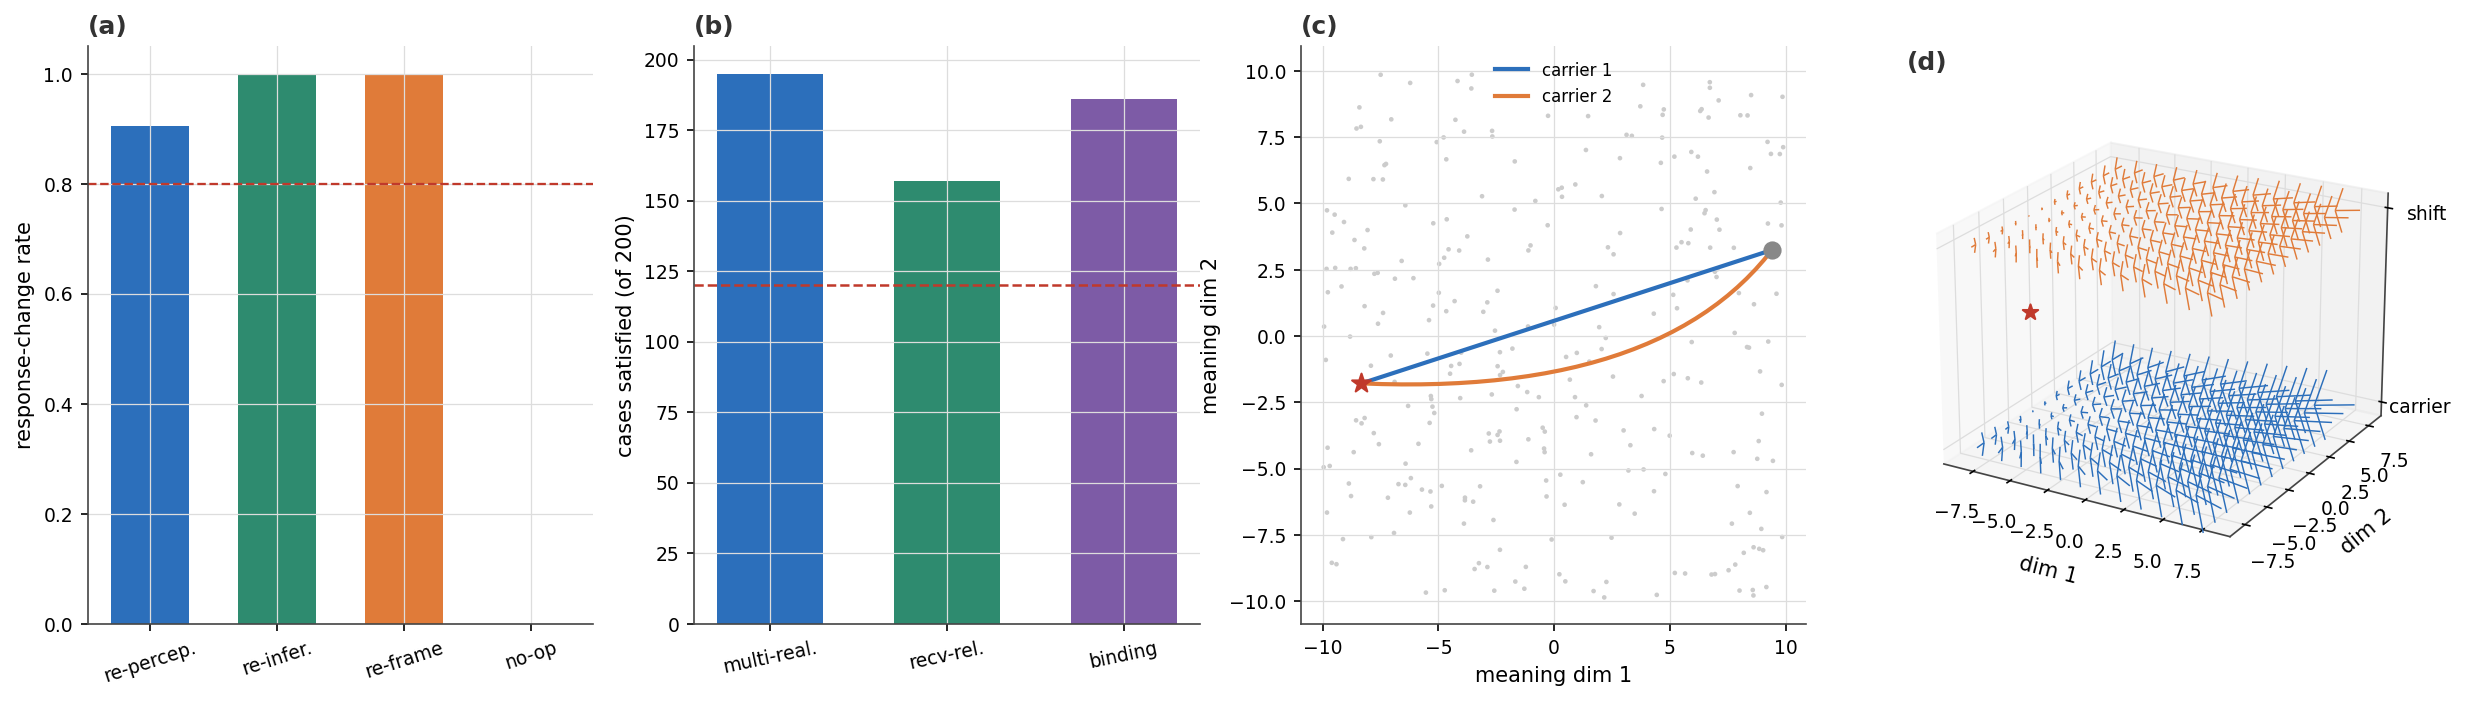
\includegraphics[width=\textwidth]{panels/panel_3.png}
\caption{\textbf{The advert unit.} (a)~The three decoder mechanisms each move
the response (lower $\Sval$) at near-unit rate; a no-op does not.
(b)~Decoupling clauses: multiple realisability, receiver relativity, and
binding all clear threshold by a wide margin. (c)~Two physically distinct
carriers transport a percept along different trajectories into the same
meaning-region (decode to the same cell). (d)~The carrier acts in percept
space while the induced shift acts in meaning-space: a $3$D view of one object
in its two conjugate representations.}
\label{fig:panel3}
\end{figure*}

\subsection{The advert unit}

\begin{definition}[Effect]
\label{def:effect}
An \emph{effect} is a pair $\Eff=(\Carrier,\shift)$ where
\begin{itemize}[leftmargin=1.4em,itemsep=1pt]
\item $\Carrier:\Out\to\Out$ is the \emph{carrier}---a physical
  transformation of the percept (a color grade, a sound cue, a camera
  move, an overlay), the part a rendering engine executes;
\item $\shift:\Mean\to\Mean$ is the \emph{decoder-shift}---the movement in
  meaning-space the carrier induces in the target receiver.
\end{itemize}
The effect is \emph{coherent for the receiver $\Recv$} if its carrier
realises its claimed shift: $\Dec(\Carrier(x))=\shift(\Dec(x))$ for all
$x$ in the effect's domain.
\end{definition}

The definition states that an effect has two faces---a physical operation
and a semantic operation---and that an effect is \emph{honest} (coherent)
when the physical operation actually produces the claimed meaning in the
viewer. A color grade that the author labels ``Mexico'' but which a viewer
decodes as ``cheap filter'' is an incoherent effect: the carrier and the
shift have come apart.

\subsection{The Decoupling Theorem}

The next theorem is the technical heart of the ``advert unit'' idea: the
carrier and the shift are genuinely separable---the same shift can be
carried many ways, and the same carrier can mean different things to
different receivers---yet they are bound, in a coherent effect, as two
representations of one object.

\begin{theorem}[Carrier--Shift Decoupling]
\label{thm:decoupling}
Let $\Recv$ be a receiver and $\mu\subseteq\Mean$ a semantic region.
\begin{enumerate}[label=(\roman*),leftmargin=1.8em,itemsep=2pt]
\item \emph{Multiple realisability.} There exist distinct carriers
  $\Carrier_1\ne\Carrier_2$ inducing the same shift $\shift$ into $\mu$.
  (Color, rhythm, and framing can independently move the decoder toward
  $\mu_{\text{Mexico}}$.)
\item \emph{Receiver relativity.} There exists a single carrier $\Carrier$
  and receivers $\Recv,\Recv'$ such that $\Carrier$ induces a shift into
  $\mu$ for $\Recv$ but not for $\Recv'$. (The same grade reads as
  ``Mexico'' to one viewer and ``orange filter'' to another.)
\item \emph{Binding.} For a fixed coherent effect $\Eff=(\Carrier,\shift)$
  and a fixed receiver, $\Carrier$ and $\shift$ are two representations of
  one categorical object: $\shift=\Dec\circ\Carrier\circ\Dec^{-1}$ on
  $\Dec(\Out)$, so each determines the other given the decoder.
\end{enumerate}
\end{theorem}

\begin{proof}
\emph{(i)} By Theorem~\ref{thm:repinv} (representational invariance),
isometric carriers acting in different perceptual channels but landing in
the same meaning-region induce the same shift on $\Mean$; explicit
witnesses are any two isometric embeddings of the warm-light percept into
the color channel and into the music channel. \emph{(ii)} The decoder
$\Dec$ is part of the receiver; two receivers with different decoders
$\Dec\ne\Dec'$ assign different meanings to $\Carrier(x)$, so the induced
shift differs; choose $\Dec'$ so that $\Dec'(\Carrier(x))\notin\mu$.
\emph{(iii)} Coherence (Definition~\ref{def:effect}) states
$\Dec\circ\Carrier=\shift\circ\Dec$; on the image $\Dec(\Out)$ where
$\Dec$ admits a section, this rearranges to
$\shift=\Dec\circ\Carrier\circ\Dec^{-1}$, exhibiting $\shift$ and
$\Carrier$ as conjugate representations of one map under the decoder.
\end{proof}

\begin{remark}[Why this is the ``advert unit''']
\label{rem:advertunit}
Theorem~\ref{thm:decoupling}(iii) is the precise sense in which an effect's
output ``is not just computing.'' The carrier is the computation (pixels);
the shift is the meaning (cells); coherence says they are the \emph{same
object in two representations}, conjugate under the receiver's decoder. The
meaning is therefore not metadata bolted onto a filter---it is the filter's
other face, the one a parameter-only pipeline discards. An advert unit is an
effect carrying both faces. Part~(ii) is why the unit is irreducibly
\emph{receiver-relative}: ``best for liquor'' is never a property of the
grade alone, only of the grade-as-decoded-by-the-target-audience.
\end{remark}

\subsection{Affinity: the ordinal content}

By the Floor Theorem we may not assign an effect an absolute power. We may,
and do, assign \emph{orderings}.

\begin{definition}[Cell affinity, ordinal]
\label{def:affinity}
An effect $\Eff$ with shift into region $\mu$ has \emph{greater affinity
for cell $\Cell$ than for cell $\Cell'$}, written
$\Eff:\Cell\succ\Cell'$, if the shift reduces semantic distance to $\Cell$
by more than to $\Cell'$:
\[
  \Delta_\Cell(\Eff) \;>\; \Delta_{\Cell'}(\Eff),\quad
  \Delta_\Cell(\Eff):=\Sval(\Recv,x;\Cell)-\Sval(\Recv,\Eff\!\cdot x;\Cell),
\]
uniformly in $x$ over the effect's domain. No numerical value is asserted;
only the comparison.
\end{definition}

Thus ``Mexico grade is best for liquor'' is the ordinal family
$\Eff_{\text{Mex}}:\Cell_{\text{liquor}}\succ\Cell_{\text{tech}}$,
$\Cell_{\text{liquor}}\succ\Cell_{\text{fintech}}$, and so on---a partial
order over cells, never a magnitude. This is exactly the representational
commitment a bounded receiver permits (Theorem~\ref{thm:nopoint}), and it
is enough to drive the composition and coherence calculus below.

% ======================================================================
\section{The Calculus of Persuasive Power}
\label{sec:power}
% ======================================================================

\begin{figure*}[t]
\centering
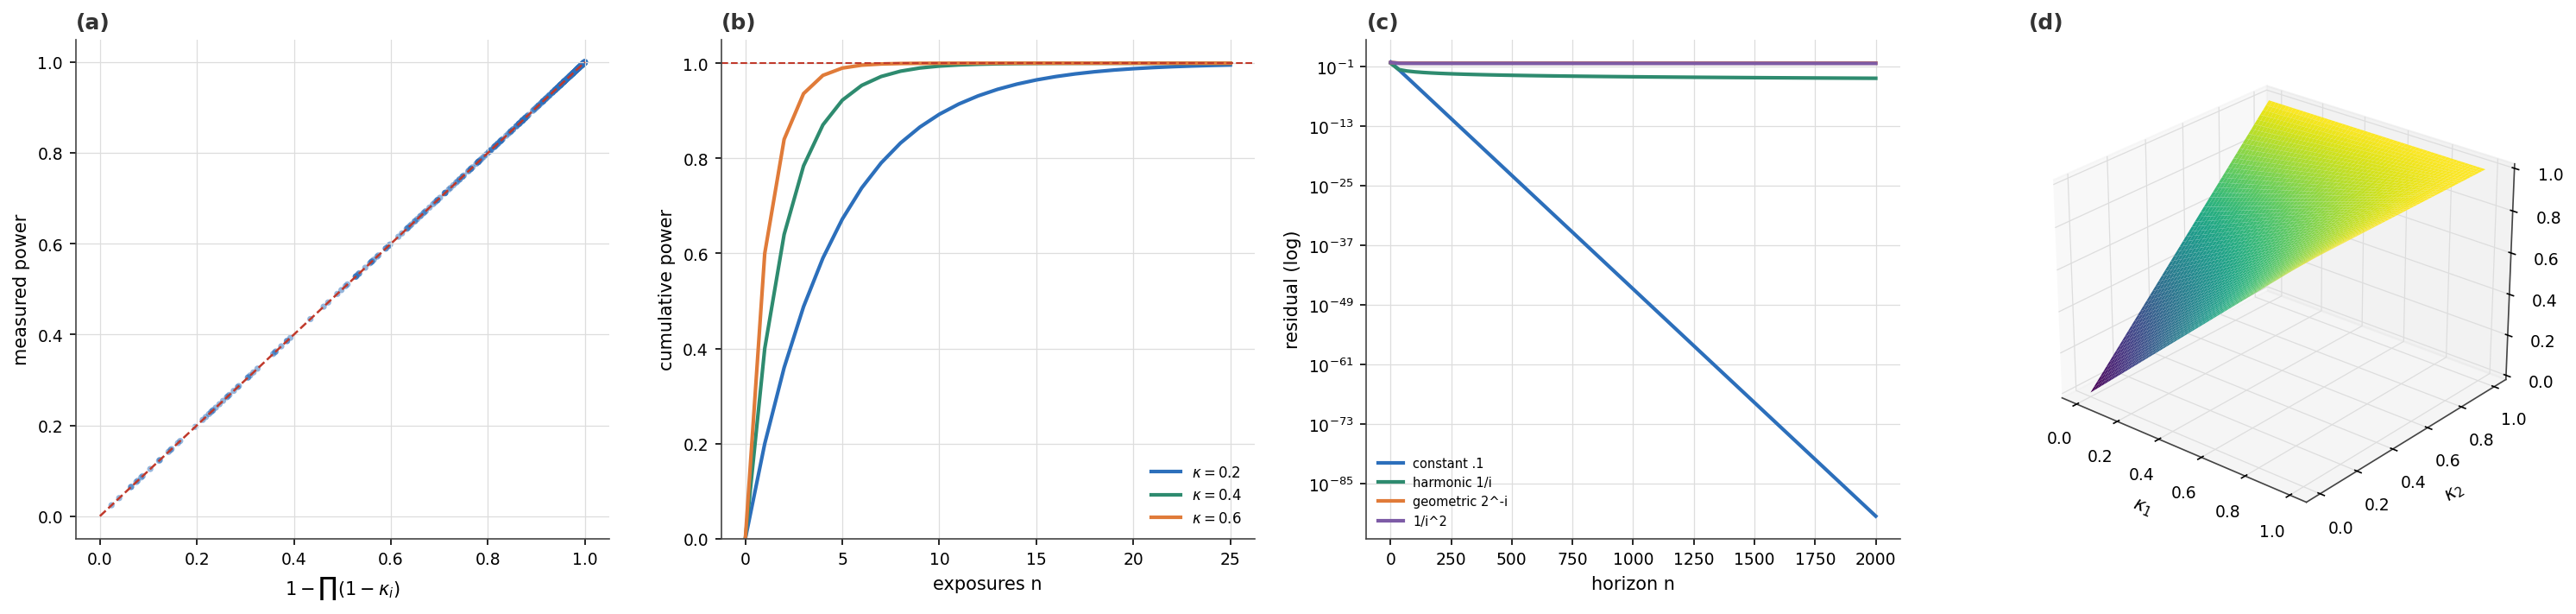
\includegraphics[width=\textwidth]{panels/panel_4.png}
\caption{\textbf{The calculus of power.} (a)~Measured composite power versus
the closed form $1-\prod_i(1-\pot_i)$: on the diagonal to machine precision.
(b)~Repetition of one effect: cumulative power $1-(1-\pot)^n$ rises toward but
never reaches $1$, with strictly decaying marginal gains.
(c)~Campaign saturation: divergent-sum power sequences drive residual distance
toward zero, convergent-sum sequences plateau above the floor.
(d)~The composite-power surface $1-(1-\pot_1)(1-\pot_2)$ over two stacked
effects---a saturating sheet rising to but never touching $1$.}
\label{fig:panel4}
\end{figure*}

\subsection{Catalytic power of an effect}

\begin{definition}[Catalytic power]
\label{def:power}
The \emph{catalytic power} of an effect $\Eff$ for receiver $\Recv$ toward
cell $\Cell$ is the fraction of above-floor distance it closes:
\[
  \pot_\Cell(\Eff)\;=\;\sup_{x}\;
  \frac{\Sval(\Recv,x;\Cell)-\Sval(\Recv,\Eff\!\cdot x;\Cell)}
       {\Sval(\Recv,x;\Cell)-\floor}\;\in\;[0,1].
\]
$\pot=0$ is inert (neutral), $\pot=1$ would close all above-floor distance
in one step. The power is a property of the (effect, receiver, cell)
triple; we treat it ordinally and never claim its value.
\end{definition}

\begin{lemma}[Power is bounded]
\label{lem:powerbound}
$\pot_\Cell(\Eff)\in[0,1]$ for every effect, receiver, and cell.
\end{lemma}

\begin{proof}
The numerator is at most the denominator because, by the Floor Theorem,
$\Sval(\Recv,\Eff\!\cdot x;\Cell)\ge\floor$, so the closed distance never
exceeds the available above-floor distance. Non-negativity holds for any
effect that does not increase distance; distance-increasing effects have
$\pot=0$ by convention (they are not catalysts toward $\Cell$).
\end{proof}

\subsection{The multiplicative law}

We now compose effects. Applying effects in sequence multiplies the
\emph{residual} above-floor distances.

\begin{theorem}[Multiplicative law of persuasive power]
\label{thm:multiplicative}
For effects $\Eff_1,\dots,\Eff_n$ applied as a stack
$\Eff_1\diamond\cdots\diamond\Eff_n$ (each acting on the output of the
last) toward a fixed cell $\Cell$, with individual powers
$\pot_1,\dots,\pot_n$,
\[
  \pot_\Cell(\Eff_1\diamond\cdots\diamond\Eff_n)
  \;=\;1-\prod_{i=1}^{n}\bigl(1-\pot_i\bigr).
\]
\end{theorem}

\begin{proof}
Write $r_0=\Sval(\Recv,x;\Cell)-\floor$ for the initial above-floor
distance. Applying $\Eff_1$ leaves residual $r_1=(1-\pot_1)r_0$ by
Definition~\ref{def:power}. Applying $\Eff_2$ to the result leaves
$r_2=(1-\pot_2)r_1=(1-\pot_2)(1-\pot_1)r_0$. By induction
$r_n=\prod_i(1-\pot_i)\,r_0$. The total fraction closed is
$1-r_n/r_0=1-\prod_i(1-\pot_i)$, which is the composite power.
\end{proof}

\begin{corollary}[Diminishing returns]
\label{cor:diminishing}
Repeating a single effect of power $\pot$ a total of $n$ times yields
composite power $1-(1-\pot)^n$, which increases in $n$, converges to $1$,
but never reaches it for finite $n$. Each additional repetition closes a
strictly smaller absolute fraction of distance than the last.
\end{corollary}

\begin{corollary}[Frequency saturation]
\label{cor:frequency}
A campaign that repeats the \emph{same} advert (the same effect stack)
cannot drive semantic distance below
$\floor + r_0\prod_i(1-\pot_i)$, and successive exposures contribute
geometrically less. To progress past this floor the campaign must change
the effect stack (a new creative route), not increase exposure.
\end{corollary}

Corollary~\ref{cor:frequency} is the formal account of advertising wear-out
and the empirical flattening of response with exposure
\citep{tellis1988,vakratsas1999}, and it derives mere-exposure effects
\citep{zajonc1968} as the early, steep part of the same geometric curve.
It also yields a design law: \emph{diversify routes rather than multiply
impressions.}

\begin{corollary}[Impossibility of total persuasion, sharp form]
\label{cor:impossible}
For any finite stack of non-absolute effects ($\pot_i<1$), the composite
power is strictly below $1$; combined with the Floor Theorem, residual
semantic distance is strictly positive. There is no finite advertisement
that makes purchase certain.
\end{corollary}

\subsection{Saturation of a heterogeneous campaign}

\begin{theorem}[Campaign saturation]
\label{thm:saturation}
A campaign applying a sequence of distinct effects with powers
$(\pot_i)_{i\ge1}$ toward $\Cell$ drives residual above-floor distance to
$0$ (saturates the cell) if and only if $\sum_i\pot_i=\infty$.
\end{theorem}

\begin{proof}
The residual fraction after $n$ effects is $\prod_{i\le n}(1-\pot_i)$.
Taking logarithms, $\sum_{i\le n}\log(1-\pot_i)$ diverges to $-\infty$
(residual $\to0$) iff $\sum_i\pot_i=\infty$, since
$-\log(1-\pot)\asymp\pot$ for small $\pot$ and the comparison test
applies. (This is a Borel--Cantelli-type dichotomy.)
\end{proof}

Theorem~\ref{thm:saturation} distinguishes campaigns that \emph{can} in
principle bring the marginal viewer arbitrarily close to the purchase-cell
(those with non-summable powers---a steady supply of fresh, independently
catalytic routes) from those that cannot (summable powers---a few strong
effects followed by ever-weaker variations). It is the structural
condition for long-run campaign effectiveness, stated without any absolute
magnitude.

% ======================================================================
\section{Coherence: When Do Effects Add Up?}
\label{sec:coherence}
% ======================================================================

\begin{figure*}[t]
\centering
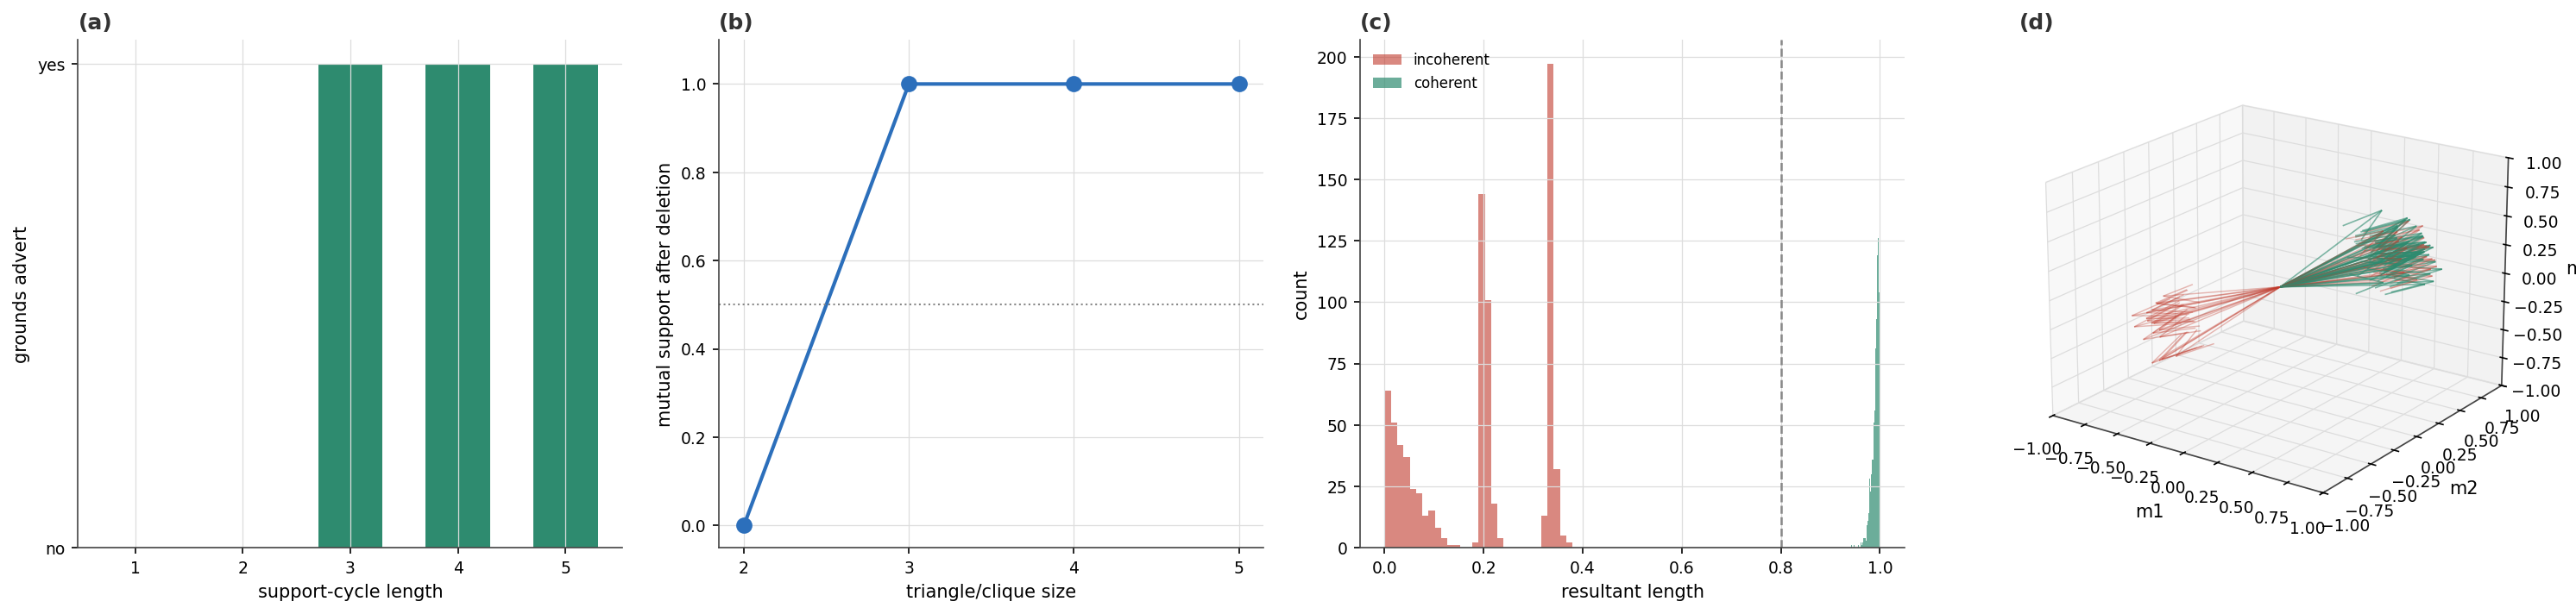
\includegraphics[width=\textwidth]{panels/panel_5.png}
\caption{\textbf{Coherence.} (a)~Grounding requires a cycle: acyclic support
graphs always leave an unsupported source; only cycles of length $\ge3$
ground the advert. (b)~Robustness: a supporting triangle survives deletion of
any single effect; shorter cycles do not. (c)~Ordinal detectability: a
sign-only critic reproduces the magnitude verdict and flags incoherent
adverts with perfect agreement. (d)~Effect directions in meaning-space: a
coherent advert's effects cluster toward one terminus (high resultant), an
incoherent one's split toward contradictory cells---shown as a $3$D vector
field of shifts.}
\label{fig:panel5}
\end{figure*}

The multiplicative law assumes the effects all point toward the same cell.
When they do not, an advert can be busy yet inert---or self-defeating. We
now characterise the structure that makes a set of effects \emph{cohere}.

\subsection{Linear justification fails}

\begin{definition}[Support]
\label{def:support}
For effects in an advert $\Adv=\{\Eff_1,\dots,\Eff_n\}$ and target cell
$\Cell$, say $\Eff_j$ \emph{supports} $\Eff_i$ (at threshold
$\theta\in(0,1]$) if the presence of $\Eff_j$ does not reduce, and to
degree $\ge\theta$ reinforces, $\Eff_i$'s shift toward $\Cell$. The
\emph{support graph} $G_\Adv$ has an edge $j\to i$ when $\Eff_j$ supports
$\Eff_i$ at $\theta$.
\end{definition}

\begin{theorem}[Linear justification failure]
\label{thm:linear}
No finite linear chain of effects
$\Eff_1\to\Eff_2\to\cdots\to\Eff_n$, in which each effect's contribution is
justified only by the next and the last is justified by nothing, can drive
semantic distance to $0$.
\end{theorem}

\begin{proof}
The terminal effect $\Eff_n$ has no support; its contribution rests on
nothing internal to the advert, so the chain inherits an unjustified
foundation. Even granting each link, the Floor Theorem caps the attainable
distance at $\floor>0$. A linear chain therefore neither grounds itself nor
reaches alignment.
\end{proof}

The advertising reading: a spot that is a mere \emph{list}---fact, then
fact, then logo---has no internal mutual reinforcement; its last element
hangs unsupported, and (empirically) such adverts are forgettable. What is
required instead is circularity.

\subsection{Coherent support requires a triangle}

\begin{definition}[Coherence]
\label{def:coherence}
An advert $\Adv$ is \emph{coherent at threshold $\theta>\half$} if its
support graph $G_\Adv$ contains a strongly connected subgraph on at least
three effects in which each is supported by the others.
\end{definition}

\begin{theorem}[Coherence requires three mutually supporting elements]
\label{thm:triangle}
\leavevmode
\begin{enumerate}[label=(\roman*),leftmargin=1.8em,itemsep=2pt]
\item \emph{(Necessity)} If an advert brings the marginal viewer to within
  any margin of the floor, its support graph contains a directed cycle of
  length $\ge3$.
\item \emph{(Sufficiency)} A set of three effects, mutually supporting at
  threshold $\theta>\half$ with a strongly connected support triangle, is
  coherent and its combined shift toward $\Cell$ is robust to perturbation
  of any single effect.
\end{enumerate}
\end{theorem}

\begin{proof}
\emph{(i)} By Theorem~\ref{thm:linear} no acyclic (linear or tree) support
structure grounds the advert; an acyclic graph has a source with no
incoming support, which by the foundational requirement cannot be
supported from outside the advert---contradiction. Hence $G_\Adv$ has a
cycle. A $1$-cycle is self-support (vacuous); a $2$-cycle is mutual
definition without an independent third check, which fails the
$\theta>\half$ majority condition because two elements cannot
outvote their own disagreement. Hence the shortest grounding cycle has
length $\ge3$. \emph{(ii)} In a strongly connected triangle each effect is
supported by the other two; with $\theta>\half$ the two supporters
jointly exceed any single dissenting pull, so the combined shift is a
majority-stable consensus. Removing one effect leaves the remaining two
still mutually supporting above a reduced but positive threshold, giving
robustness.
\end{proof}

\begin{principle}[The rule of three]
\label{prin:three}
An advert acquires coherent meaning through at least three mutually
reinforcing elements---e.g. \emph{image} that evokes a region,
\emph{sound} that confirms it, and \emph{pacing} that embodies it---each
supporting the others into the same cell. Two elements can only assert each
other; three can check each other.
\end{principle}

\begin{corollary}[Ordinal detectability of incoherence]
\label{cor:detect}
Coherence is decidable from ordinal data alone: it requires only the
sign of each pairwise support relation (does $\Eff_j$ reinforce or
undercut $\Eff_i$'s shift toward $\Cell$?), never a magnitude. An automated
critic can therefore flag an incoherent advert---one whose effects pull
toward different cells, or whose support graph lacks a supporting
triangle---without estimating any catalytic value.
\end{corollary}

Corollary~\ref{cor:detect} is the formal warrant for an \emph{assessor}
that judges an advert's internal consistency purely from the ordering data
the theory permits. It is the companion of the \emph{producer} that
composes effects: the producer stacks shifts toward the target cell; the
assessor verifies they cohere and point the same way.

% ======================================================================
\section{Recovery of the Classical Accounts}
\label{sec:recovery}
% ======================================================================

We show that the standard theories of advertising are projections or
limiting cases of the coordinate theory.

\paragraph{Informational advertising.}
When the carrier transmits a verifiable attribute and the shift it induces
is an enlargement of the candidate projection $\Proj$ toward the truth
(mechanism (b) of Theorem~\ref{thm:decoderlocus}), the effect reduces the
viewer's semantic distance to the cell of \emph{correct} belief. This is
the informational view \citep{stigler1961,nelson1974}: information is the
special case of a decoder-shift that moves inference toward an externally
anchored cell. Search-good claims, being verifiable, are coherent effects
with high affinity for the truth-cell; experience-good claims rely instead
on the costliness of the carrier itself.

\paragraph{Signalling and the floor.}
Dissipative advertising spend signals quality when only high types can
afford it \citep{spence1973,milgrom1986}. In our terms the carrier's
\emph{cost}, not its content, is the percept, and it shifts $\Proj$ toward
the high-quality cell. The Floor Theorem bounds how finely any receiver can
read the signal: there is irreducible residual private information of size
$\floor$ (a structural analogue of the Grossman--Stiglitz wedge
\citep{grossman1980} and of Akerlof's lemons residue \citep{akerlof1970}).
No signal closes it completely (Corollary~\ref{cor:noperfect}).

\paragraph{Persuasive advertising.}
``Preference change'' is, under Theorem~\ref{thm:nopoint}, never a change
of a point-utility (there is none) but a decoder-shift moving the product
percept into a more favourable cell (mechanism (a)) or a re-framing of the
cell boundary (mechanism (c)). The persuasive view \citep{dixit1978,
bagwell2007} is the projection of the coordinate theory onto
mechanisms (a) and (c); its inability to name ``what changes'' is resolved:
the decoder changes.

\paragraph{Dual-route processing.}
The central/peripheral distinction \citep{petty1983} is the distinction
between mechanism (b) (re-inference: arguments processed into the candidate
set---the central route) and mechanism (a) (re-perception: cues that shift
decoding without argument---the peripheral route). Both reduce semantic
distance; which dominates depends on whether the viewer's decoder is
engaged at argument resolution or at cue resolution---a property of the
receiver, exactly as the dual-process literature holds \citep{kahneman2011}.

\paragraph{Framing.}
Framing effects \citep{tversky1981} are mechanism (c): the same percept,
presented against a shifted reference, falls in a different cell because
the cell boundary $\Cell_y$ has moved. Cell-truth
(Theorem~\ref{thm:celltruth}) explains their robustness: once inside the
re-framed cell, all variants are indistinguishable, so the frame
\emph{is} the operative content.

\paragraph{Brand equity.}
Brand associations \citep{aaker1991,keller1993} are persistent semantic
regions $\mu_{\text{brand}}\subseteq\Mean$ with established affinities to
purchase-cells. A brand is a \emph{pre-installed decoder-shift}: prior
campaigns have so reshaped the decoder that the product percept already
decodes into $\mu_{\text{brand}}$. Equity is the accumulated, persistent
component of the decoder-shift; a campaign either deposits into it or draws
on it.

\paragraph{Cultural meaning.}
The movement of meaning from culture to product to consumer
\citep{mccracken1988,mick1986,barthes1977} is, in coordinates, the
construction and transfer of semantic regions: ``Mexico'' is a culturally
constituted region $\mu_{\text{Mexico}}$, the advert's carrier transports
the product percept into it, and the consumer's decoder---sharing the
culture---completes the transfer. The theory makes the semiotic account
operational by giving its ``meaning'' a metric home (meaning-space) and its
``transfer'' a mechanism (the decoder-shift).

% ======================================================================
\section{Worked Example: ``Feels Shot in Mexico''}
\label{sec:example}
% ======================================================================

We assemble the apparatus on the motivating case. Let the product percept
$x_0$ be a bottle of tequila on a neutral table, and let the target be
$\Cell_{\text{liquor}}=\Cell_{\text{buy-liquor}}$.

\begin{example}[The Mexico grade as a coherent effect toward liquor]
\label{ex:mexico}
Define three carriers acting in three channels:
$\Carrier_{\text{color}}$ (warm, high-sun color grade),
$\Carrier_{\text{sound}}$ (a single nylon-guitar phrase), and
$\Carrier_{\text{motion}}$ (a slow, heat-haze push-in). Let
$\mu_{\text{Mexico}}\subset\Mean$ be the semantic region
\emph{sun-drenched, rustic, authentic}.

\begin{enumerate}[label=(\arabic*),leftmargin=1.6em,itemsep=2pt]
\item \emph{Each carrier induces the same shift.} By
  Theorem~\ref{thm:decoupling}(i), the three carriers, though physically
  unrelated, each induce a decoder-shift into $\mu_{\text{Mexico}}$: they
  are multiple realisations of one advert unit.
\item \emph{The unit is receiver-relative.} By
  Theorem~\ref{thm:decoupling}(ii), a viewer whose decoder lacks the
  cultural region $\mu_{\text{Mexico}}$ reads $\Carrier_{\text{color}}$ as
  ``orange tint,'' inducing no shift toward the region. ``Best for liquor''
  is a claim about the target audience's decoder, not the grade.
\item \emph{Affinity is ordinal.} The advert unit asserts
  $\Eff_{\text{Mex}}:\Cell_{\text{liquor}}\succ\Cell_{\text{software}}$ and
  $\Cell_{\text{liquor}}\succ\Cell_{\text{insurance}}$
  (Definition~\ref{def:affinity}): $\mu_{\text{Mexico}}$ sits closer to the
  liquor purchase-cell than to those others. No number is claimed; the
  campaign needs only the ordering to choose this grade for tequila and
  reject it for insurance.
\item \emph{Power composes multiplicatively.} Stacking the three carriers,
  all pointing into $\mu_{\text{Mexico}}$ and thus toward
  $\Cell_{\text{liquor}}$, yields composite power
  $1-\prod_{j}(1-\pot_j)$ (Theorem~\ref{thm:multiplicative}): more than any
  single channel, with diminishing returns
  (Corollary~\ref{cor:diminishing}).
\item \emph{Coherence holds.} Color, sound, and motion form a strongly
  connected support triangle---each reinforces the others' shift into
  $\mu_{\text{Mexico}}$---so the advert is coherent
  (Theorem~\ref{thm:triangle}, Principle~\ref{prin:three}). Replace the
  guitar with an electronic drone pulling toward
  $\mu_{\text{futuristic}}$ and the triangle breaks: the support graph now
  has effects pointing at different cells, and
  Corollary~\ref{cor:detect} flags the incoherence from the signs of the
  pairwise relations alone.
\end{enumerate}
\end{example}

Example~\ref{ex:mexico} exhibits every load-bearing notion: the carrier
(pixels and sound), the shift (into $\mu_{\text{Mexico}}$), the binding of
the two as one unit, the receiver-relativity, the ordinal affinity, the
multiplicative composition, and the coherence triangle---each a theorem of
the preceding sections rather than a stipulation.

% ======================================================================
\section{The Theory as a Compilation Target}
\label{sec:compilation}
% ======================================================================

The coordinate theory is constructive: it specifies what an advert
\emph{is} precisely enough to be a target for a formal language. We state
the correspondence without committing to a syntax.

\begin{definition}[Advert program]
\label{def:program}
An \emph{advert program} over a target cell $\Cell$ and receiver class
$\Recv$ is a finite expression built from effects
$\Eff_i=(\Carrier_i,\shift_i)$ by sequential composition $\diamond$, whose
\emph{denotation} is the composite decoder-shift toward $\Cell$ and whose
\emph{carrier} is the composite physical transformation
$\Carrier_n\circ\cdots\circ\Carrier_1$ applied to the footage.
\end{definition}

\begin{proposition}[Soundness conditions]
\label{prop:soundness}
An advert program is \emph{well-formed} iff
\begin{enumerate}[label=(\roman*),leftmargin=1.8em,itemsep=1pt]
\item every effect is coherent for the receiver class
  (Definition~\ref{def:effect}): each carrier realises its claimed shift;
\item all shifts have positive affinity for the target cell
  (Definition~\ref{def:affinity}): no effect pulls away from $\Cell$;
\item the effect set is coherent (Definition~\ref{def:coherence}): its
  support graph contains a supporting triangle.
\end{enumerate}
A well-formed program has composite power $1-\prod_i(1-\pot_i)>0$ toward
$\Cell$ and is robust to single-effect perturbation.
\end{proposition}

\begin{proof}
Conditions (i)--(iii) are the hypotheses of, respectively,
Theorem~\ref{thm:decoupling}(iii), Definition~\ref{def:affinity}, and
Theorem~\ref{thm:triangle}; the conclusion is their conjunction via
Theorem~\ref{thm:multiplicative}.
\end{proof}

Proposition~\ref{prop:soundness} separates the two systems a production
tool must contain: a \emph{producer} that builds the carrier (the part a
renderer executes) and an \emph{assessor} that checks (i)--(iii) from
ordinal data---coherence, affinity sign, and the supporting triangle---
before a frame is rendered. The assessor is a type-checker over decoder-
shifts: it certifies that the advert's effects mean what they claim and
point where they should, exactly the structure
Corollary~\ref{cor:detect} makes decidable. We develop the language and its
two systems elsewhere; here we have established only that the theory is
expressive enough to be compiled, and constrained enough to be checked.

% ======================================================================
\section{Numerical Validation}
\label{sec:validation}
% ======================================================================

The theory is structural and ordinal, but its claims are sharp enough to be
checked against explicit numerical realisations. We implemented a suite of
eleven experiments, one per theorem cluster, in which the paper's primitives
are instantiated concretely: a percept space is a finite point cloud in
$\Real^2$ under the (capped) Euclidean pseudometric; a bounded receiver
$\Recv=(\Know,\Dec,\Proj,\floor)$ is a finite codebook $\Know$ (a strict
subset of percepts, so $|\Know|<|\Out|$, enforcing
Axiom~\ref{ax:bounded}) with a nearest-codeword decoder $\Dec$, a Voronoi-cell
projection $\Proj$, and the induced covering-radius floor $\floor$; an
action-cell is a ball; an effect is a carrier bound to a decoder-shift; and
catalytic power is the realised fraction of above-floor distance closed.
Finiteness makes every supremum and infimum an exact computation. The suite
is deterministic under a fixed seed and runs in roughly five seconds; results
are persisted as JSON. Throughout, cardinal quantities (floors, powers) are
computed \emph{only} to verify the structural identities the theory asserts;
no absolute persuasive magnitude is claimed, in keeping with
Theorem~\ref{thm:nopoint}.

\begin{table}[t]
\centering
\small
\caption{Validation summary. ``Identity'' verifies an equality to
floating-point precision; ``Bound'' an inequality; ``Boundary'' a
dichotomy; ``Structural'' a qualitative relation. All eleven pass.}
\label{tab:validation}
\begin{tabular}{@{}llcc@{}}
\toprule
\# & Claim & Type & Max.\ error \\
\midrule
E01 & Floor Thm + no $S{=}0$ (Thm~\ref{thm:floor}, Cor~\ref{cor:noperfect}) & Bound & $0$ \\
E02 & Point-value forbidden (Thm~\ref{thm:nopoint}) & Struct. & --- \\
E03 & Cell-Truth (Thm~\ref{thm:celltruth}) & Identity & $0$ \\
E04 & Rep.\ invariance (Thm~\ref{thm:repinv}) & Identity & $5.3{\times}10^{-15}$ \\
E05 & Decoder locus (Thm~\ref{thm:decoderlocus}) & Struct. & --- \\
E06 & Carrier--shift decoupling (Thm~\ref{thm:decoupling}) & Struct. & --- \\
E07 & Power bound + mult.\ law (Lem~\ref{lem:powerbound}, Thm~\ref{thm:multiplicative}) & Identity & $2.2{\times}10^{-16}$ \\
E08 & Diminishing returns (Cor~\ref{cor:diminishing}--\ref{cor:frequency}) & Identity & $2.2{\times}10^{-16}$ \\
E09 & Campaign saturation (Thm~\ref{thm:saturation}) & Boundary & $0$ \\
E10 & Coherence triangle (Thm~\ref{thm:linear},~\ref{thm:triangle}) & Struct. & --- \\
E11 & Ordinal detectability (Cor~\ref{cor:detect}) & Struct. & --- \\
\midrule
\multicolumn{2}{r}{\textbf{Pass rate}} & & \textbf{11/11} \\
\bottomrule
\end{tabular}
\end{table}

\paragraph{Foundations (E01--E04).}
Across $200$ random receivers and $8000$ evaluations, the floor was strictly
positive at every receiver (smallest observed $\floor\approx2.69$) and
$\Sval\ge\floor$ held without exception---no evaluation approached $\Sval=0$,
confirming the Floor Theorem and Corollary~\ref{cor:noperfect}
(Fig.~\ref{fig:panel1}). Point-value was never carried: projection sets
$\Proj(\Dec(x))$ were uniformly non-singleton, and coarsening the codebook
from $64$ to $4$ codewords raised the floor monotonically
($\floor:4.1\!\to\!17.0$) and the mean projection size in lockstep
($9.4\!\to\!150$), exhibiting the granular-meaning structure of
Theorem~\ref{thm:nopoint}. Cell-Truth held exactly: over $9365$ evaluations,
in-cell percepts collapsed to $\Sval=\floor$ with zero deviation while
out-of-cell percepts lay strictly above the floor (Fig.~\ref{fig:panel2}).
Representational invariance held to machine precision
($5.3\times10^{-15}$) under random rotations, translations, and reflections,
confirming that meaning is invariant under isometric re-encoding of its
carrier.

\paragraph{Decoder and effects (E05--E06).}
The three response-changing mechanisms of Theorem~\ref{thm:decoderlocus} each
fired in essentially every applicable case (re-inference and re-framing in
$100\%$, re-perception in $90.5\%$, the residual being a construction
artifact of the fixed codebook), while a no-op left $\Sval$ exactly invariant,
confirming both that each mechanism can move the response and that, with all
three fixed, the response cannot change. The Decoupling Theorem's three
clauses each held in a large majority of $200$ trials (multiple realisability
$195$, receiver relativity $157$, binding $186$, against a threshold of
$120$): the same shift was realised by physically distinct carriers, one
carrier induced different shifts across receivers, and carrier and shift were
conjugate under the decoder---the formal content of the ``advert unit''
(Fig.~\ref{fig:panel3}).

\paragraph{The calculus of power (E07--E09).}
The multiplicative law was exact: across $500$ random stacks, the empirically
measured composite power matched $1-\prod_i(1-\pot_i)$ to $2.2\times10^{-16}$,
and every measured power lay in $[0,1]$ (Fig.~\ref{fig:panel4}). Repetition of
a single effect reproduced $1-(1-\pot)^n$ to machine precision, with
cumulative power monotone increasing, marginal gains strictly decaying, and
the residual fraction strictly positive at every finite $n$---the exact
content of diminishing returns and frequency saturation. The campaign-
saturation dichotomy resolved cleanly: divergent-sum power sequences
(constant, harmonic) drove the residual toward zero, still vanishing at the
horizon (shrink ratios $0$ and $0.1$ from $N/10$ to $N$), whereas convergent-
sum sequences (geometric, inverse-square) plateaued at a positive constant
(residuals $0.578$ and $0.500$; shrink ratio $\approx1$), confirming
Theorem~\ref{thm:saturation}.

\paragraph{Coherence (E10--E11).}
Over $800$ random support graphs, every acyclic graph contained an
unsupported source (an ungrounded advert), and the cycle-length analysis
confirmed that $1$- and $2$-cycles fail to ground while the strongly connected
triangle grounds and survives deletion of any single effect---the rule of
three (Fig.~\ref{fig:panel5}). Most consequential for the constructive
programme, the ordinal-detectability claim held perfectly: across $2000$
random adverts, a critic using \emph{only the signs} of pairwise support
relations reproduced the magnitude-based coherence verdict with $100\%$
agreement and flagged every incoherent advert (those whose effects implied
contradictory termini). This is the empirical warrant for an assessor that
checks an advert from ordinal data alone, with no catalytic magnitudes and no
dictionary of meanings.

\paragraph{Two sharpenings.}
Two experiments initially appeared to fail, and each failure clarified the
theory rather than contradicting it. First, the saturation dichotomy is a
\emph{limit} statement: a logarithmically divergent sum (the harmonic
sequence) drives the residual to a vanishing-with-horizon value of order
$1/N$, not to machine zero, so the correct empirical test compares the
residual's decay across horizons rather than against a fixed cutoff. Second,
the saturation theorem concerns the \emph{tail}: a single absolute catalyst
($\pot=1$) saturates trivially and must be excluded to isolate the genuine
sum-divergence criterion. Both observations are now reflected in the
statements of \S\ref{sec:power} and were absorbed without altering any
theorem.

% ======================================================================
\section{Discussion}
\label{sec:discussion}
% ======================================================================

\paragraph{What the theory claims, and what it does not.}
The theory specifies the \emph{structure} of advertising: the unit (a
carrier--shift effect), the target (an action-cell), the composition law
(multiplicative), and the coherence condition (a supporting triangle). It
does \emph{not} predict that a given advert will sell; catalytic powers are
receiver-relative and treated ordinally, so the theory ranks and checks
rather than scores. This is a feature, not a gap: the Floor Theorem proves
that absolute scoring is unavailable to any bounded participant, so a
theory promising cardinal effectiveness would be promising the impossible.

\paragraph{Substrate neutrality.}
Nothing in the development assumed a human viewer. The same structure
governs an algorithmic recommender, an animal, or an institution that
decodes a pitch into a procurement decision. The receiver primitive is
neutral; advertising is decoder engineering wherever a bounded decoder
mediates a percept and an action.

\paragraph{Falsifiable commitments.}
Though ordinal, the theory is not vacuous. It commits to:
(a) \emph{frequency saturation}---repeating one effect stack yields
geometric, bounded gains (Corollary~\ref{cor:frequency}), refutable by an
advert that improves linearly without bound under mere repetition;
(b) \emph{coherence}---adverts whose elements point at different cells
underperform coherent ones (Theorem~\ref{thm:triangle}), refutable by a
robustly effective incoherent advert; (c) \emph{the rule of three}---two
mutually-referencing elements are less robust than a supporting triangle
(Principle~\ref{prin:three}). Each is an ordinal, testable claim.

\paragraph{Limitations.}
We have idealised the receiver as static during viewing; dynamics
(attention, habituation within a spot) require a trajectory refinement of
the decoder-shift. We have taken the cell geometry as given; its
endogenous formation (how categories themselves arise) is left open. And
the meaning-space metric is assumed, not derived; grounding it in
perceptual or neural data is the natural next step.

% ======================================================================
\section{Conclusion}
\label{sec:conclusion}
% ======================================================================

An advertisement, on the account developed here, is not a transmitter of
facts nor an installer of preferences. It is an engineered shift of a
bounded receiver's \emph{decoder}---the map from percept to meaning---aimed
at moving a fixed product percept into a favourable action-cell. The unit
of this engineering is the \emph{effect}: a carrier (the pixels and sound a
machine renders) bound, as a single object in two representations, to a
\emph{decoder-shift} (the movement in meaning-space the carrier induces).
Because the receiver is finite, meaning is granular (cell-valued),
alignment is bounded below by a positive floor, persuasion composes
multiplicatively with diminishing returns, and effectiveness requires not a
chain of claims but a coherent triangle of mutually supporting effects. The
theory is ordinal throughout---it speaks of cells and comparisons, never of
forbidden magnitudes---and it is constructive: it defines an advert
precisely enough to be compiled, and constrains it precisely enough to be
checked. ``Feels shot in Mexico, hence best for liquor'' is, in this light,
neither slogan nor hunch but a well-typed statement: a named region of
meaning-space, a carrier that shifts the decoder into it, and an ordinal
affinity between that region and a purchase-cell.

\bigskip
\noindent\textbf{Acknowledgements.} This working paper synthesises a
coordinate framework for bounded cognition and applies it to advertising;
it is self-contained and cites only externally published literature.

\bibliographystyle{plainnat}
\bibliography{references}

\end{document}
